% !TEX program = xelatex
\documentclass[10pt,twocolumn,a4paper]{article}
\usepackage{extarrows} 
% ===== Essential Packages =====
\usepackage[T1]{fontenc}
\usepackage{lmodern}
\usepackage[UTF8, fontset=none]{ctex}
\usepackage{xeCJK}
\usepackage{enumitem}
\setCJKmainfont{Noto Serif CJK SC}
\setCJKsansfont{Noto Sans CJK SC}
\setCJKmonofont{Noto Sans Mono CJK SC}

% ===== Math & Symbols =====
\usepackage{amsmath}
\usepackage{amssymb}
\usepackage{mathrsfs}
\usepackage{braket}

% ===== Graphics & Tables =====
\usepackage{graphicx}
\usepackage{float}
\usepackage{wrapfig}
\usepackage{tikz}
\usepackage[table]{xcolor}
\usepackage{array}
\usepackage{multirow}
\usepackage{tabularx}
\usepackage{booktabs}
\usepackage{siunitx}
\usepackage{caption}
\usepackage{subcaption}
\usepackage{adjustbox}

% ===== Code Listings =====
\usepackage{listings}
\usepackage{tcolorbox}
\tcbuselibrary{listings, breakable}

% ===== Misc =====
\usepackage{lipsum}
\usepackage{footmisc}
\usepackage[margin=1in]{geometry}
\usepackage{diagbox}
\usepackage{mathtools}
\usepackage{tensor}

\lstset{
	basicstyle=\small\ttfamily,
	numbers=left,
	numberstyle=\tiny\color{gray},
	keywordstyle=\color{blue},
	commentstyle=\color{green!60!black},
	stringstyle=\color{red},
	frame=single,
	breaklines=true,
	showstringspaces=false,
	tabsize=2,
	captionpos=b
}
\author{
	张世航 \\
	学号:320230938701 \\
	\texttt{zhshihang2023@lzu.edu.cn}
}
\title{电光效应}

\begin{document}
	\maketitle
	
	\section{红正黑负}
	\subsection{拟合法}
	我们画出曲线：
	\begin{figure}[H]
		\centering
		
\includegraphics[width=0.7\linewidth]{1.png}
		\caption{蓝色为拟合曲线}
		\label{fig:1}
	\end{figure}
	
	拟合公式为：
	\begin{equation}
		P = A\sin(kU) + B\cos(kU) + b = R\cos(kU - \varphi) + b
	\end{equation}
	其中 $R = \sqrt{A^2+B^2}$，$\varphi = \arctan(B/A)$。
	利用梯度下降方法（Adam 优化器），以二次方之和为损失函数得到最佳拟合曲线。
	
	拟合得到：
	\begin{equation}
		A = -0.0113,\quad B = -0.2104,\quad k = 0.6367,\quad b = 0.2250
	\end{equation}
	\begin{equation}
		R = 0.2107,\quad \varphi = -1.6245\,\text{rad}
	\end{equation}
	
	即：
	\begin{equation}
		P = 0.2107\cos(0.6367U - 1.6245) + 0.2250
	\end{equation}
	
	利用 $\cos\alpha = 1 - 2\sin^2(\alpha/2)$：
	\begin{equation}
		\begin{aligned}
			P &= 0.2107\left[1 - 2\sin^2\left(\frac{0.6367U - 1.6245}{2}\right)\right] + 0.2250 \\
			&= 0.4357 - 0.4214\sin^2(0.31835U - 0.81225)
		\end{aligned}
	\end{equation}
	
	标准形式：
	\begin{equation}
		I = (I_{\max}^+ - I_{\min}^+)\sin^2\left(\frac{\pi\frac{U}{V_\pi^+} + \delta_0^+}{2}\right) + I_{\min}^+
	\end{equation}
	
	四个参数：
	\begin{align}
		I_{\max}^+ &= 0.4357\ \text{mW} \\
		I_{\min}^+ &= 0.0143\ \text{mW} \\
		V_\pi^+ &= 360\ \text{V} \\
		\delta_0^+ &= -1.6245\ \text{rad}
	\end{align}
	
	\begin{equation}
		M^+ = \frac{I_{\max}^+}{I_{\min}^+}=\frac{0.4357}{0.0143} = 30.47
	\end{equation}
	
	\subsection{极值法}
	对正电压扫描数据（步长 \(20\,\text{V}\)），得到光强极大值和极小值及其对应电压：
	\begin{equation}
		U_{\text{max}}^{(\text{极+})} = 380\,\text{V},\quad I_{\text{max}}^{(\text{极+})} = 0.435\,\text{mW};
	\end{equation}
	\begin{equation}
		U_{\text{min}}^{(\text{极+})} = 780\,\text{V},\quad I_{\text{min}}^{(\text{极+})} = 0.018\,\text{mW}.
	\end{equation}
	于是：
	\begin{equation}
		V_{\pi}^{(\text{极+})} = \left| U_{\text{max}}^{(\text{极+})} - U_{\text{min}}^{(\text{极+})} \right| = 400\,\text{V},
	\end{equation}
	\begin{equation}
		M^{(\text{极+})} = \frac{I_{\text{max}}^{(\text{极+})}}{I_{\text{min}}^{(\text{极+})}} = 24.17.
	\end{equation}
	
	\section{红负黑正}
	\subsection{拟合法}
	\begin{figure}[H]
		\centering
		
\includegraphics[width=0.7\linewidth]{2}
		\caption{蓝色为拟合曲线}
		\label{fig:2}
	\end{figure}
	
	拟合公式同上，得到：
	\begin{equation}
		A = 0.0488,\quad B = -0.2343,\quad k = 0.6366,\quad b = 0.2690
	\end{equation}
	\begin{equation}
		R = 0.2393,\quad \varphi = -1.3656\,\text{rad}
	\end{equation}
	
	即：
	\begin{equation}
		P = 0.2393\cos(0.6366U - 1.3656) + 0.2690
	\end{equation}
	
	化为 $\sin^2$ 形式：
	\begin{equation}
		\begin{aligned}
			P &= 0.2393\left[1 - 2\sin^2\left(\frac{0.6366U - 1.3656}{2}\right)\right] + 0.2690 \\
			&= 0.5083 - 0.4786\sin^2(0.3183U - 0.6828)
		\end{aligned}
	\end{equation}
	
	四个参数：
	\begin{align}
		I_{\max}^- &= 0.5083\ \text{mW} \\
		I_{\min}^- &= 0.0297\ \text{mW} \\
		V_\pi^- &= 389\ \text{V} \\
		\delta_0^- &= -1.3656\ \text{rad}
	\end{align}
	\begin{equation}
		M^- = \frac{I_{\max}}{I_{\min}} = \frac{0.5083}{0.0297}=17.1
	\end{equation}
	
	\subsection{极值法}
	对负电压扫描数据（步长 \(20\,\text{V}\)），得到光强极大值和极小值及其对应电压：
	\begin{equation}
		U_{\text{max}}^{(\text{极-})} = -360\,\text{V},\quad I_{\text{max}}^{(\text{极-})} = 0.510\,\text{mW};
	\end{equation}
	\begin{equation}
		U_{\text{min}}^{(\text{极-})} = -740\,\text{V},\quad I_{\text{min}}^{(\text{极-})} = 0.027\,\text{mW}.
	\end{equation}
	于是：
	\begin{equation}
		V_{\pi}^{(\text{极-})} = \left| U_{\text{max}}^{(\text{极-})} - U_{\text{min}}^{(\text{极-})} \right| = 380\,\text{V},
	\end{equation}
	\begin{equation}
		M^{(\text{极-})} = \frac{I_{\text{max}}^{(\text{极-})}}{I_{\text{min}}^{(\text{极-})}} = 18.89.
	\end{equation}
	
	\section{结果比较}\label{sec:compare}
	\subsection{拟合法}
	两种接法测得的半波电压取平均：
	\begin{equation}
		\boxed{V_\pi = 374.5\,\text{V}}
	\end{equation}
	\begin{equation}
		\boxed{M = \sqrt{M^+M^-} = 22.8}
	\end{equation}
	\begin{equation}
		\boxed{r_{22} = \frac{\lambda d}{2n_0^3 l V_{\pi}} = 6.219773031\times10^{-12}\,\text{m/V}}
	\end{equation}
	
	\subsection{极值法}
	\begin{equation}
		V_{\pi}^{(\text{极})} = \frac{V_{\pi}^{(\text{极-})} + V_{\pi}^{(\text{极+})}}{2} = 390.0\,\text{V},
	\end{equation}
	\begin{equation}
		M^{(\text{极})} = \sqrt{M^{(\text{极-})} M^{(\text{极+})}} = \sqrt{18.89 \times 24.17} = 21.36.
	\end{equation}
	电光系数计算公式为 \( r_{22} = \dfrac{\lambda d}{2 n_o^3 V_{\pi} l} \)，代入参数：
	\begin{equation}
		\boxed{r_{22}^{(\text{极})} = 6.13 \times 10^{-12}\,\text{m/V}.}
	\end{equation}
	
	\section{正弦信号电光调制特性}
	\begin{figure}[H]
		\centering
		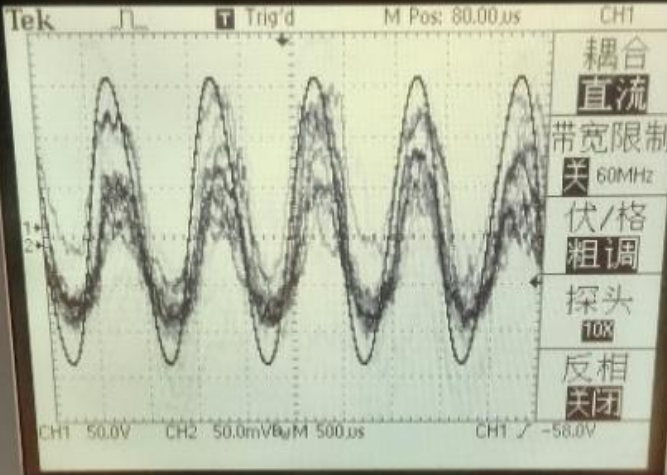
\includegraphics[width=0.7\linewidth]{38}
		\caption{$\theta=38^\circ$}
		\label{fig:38}
	\end{figure}
	
	\begin{figure}[H]
		\centering
		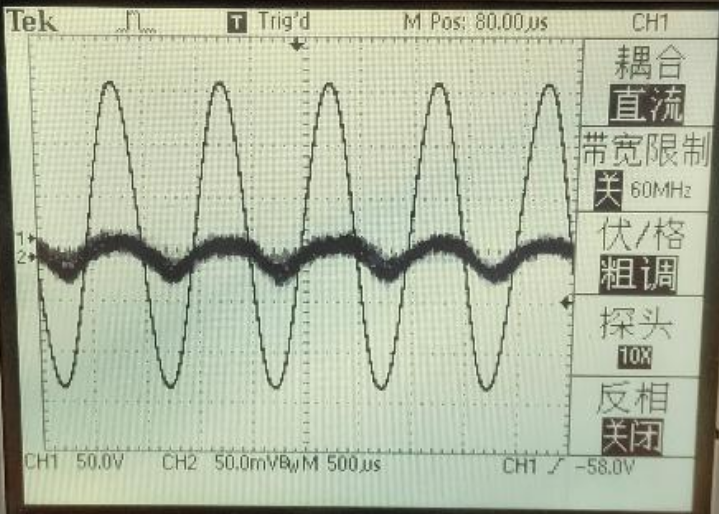
\includegraphics[width=0.7\linewidth]{98}
		\caption{$\theta=98^\circ$}
		\label{fig:98}
	\end{figure}
	\begin{figure}[H]
		\centering
		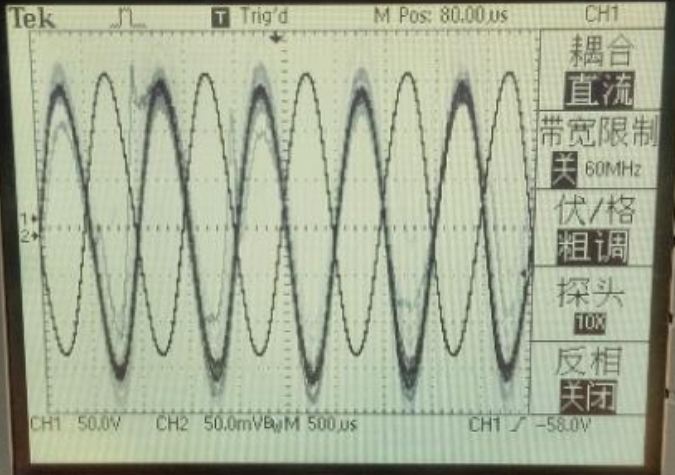
\includegraphics[width=0.7\linewidth]{126.5}
		\caption{$\theta=126.5^\circ$}
		\label{fig:126}
	\end{figure}
	\begin{figure}[H]
		\centering
		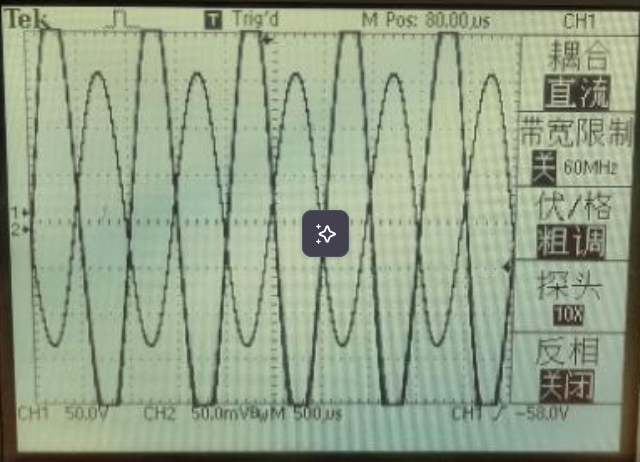
\includegraphics[width=0.7\linewidth]{162}
		\caption{$\theta=162^\circ$}
		\label{fig:162}
	\end{figure}
	\begin{figure}[H]
		\centering
		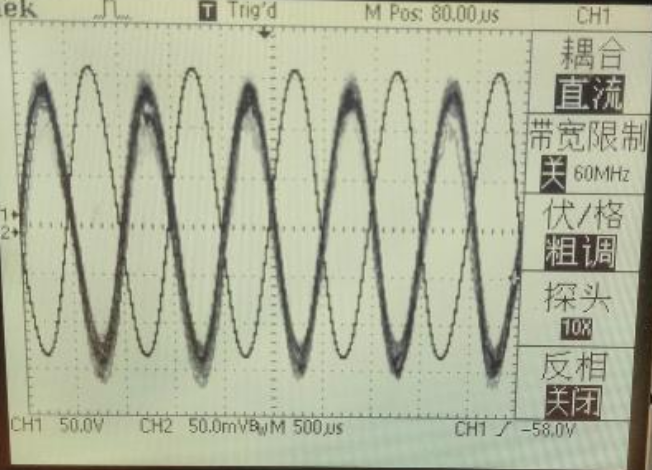
\includegraphics[width=0.7\linewidth]{200}
		\caption{$\theta=200^\circ$}
		\label{fig:200}
	\end{figure}
	\begin{figure}[H]
		\centering
		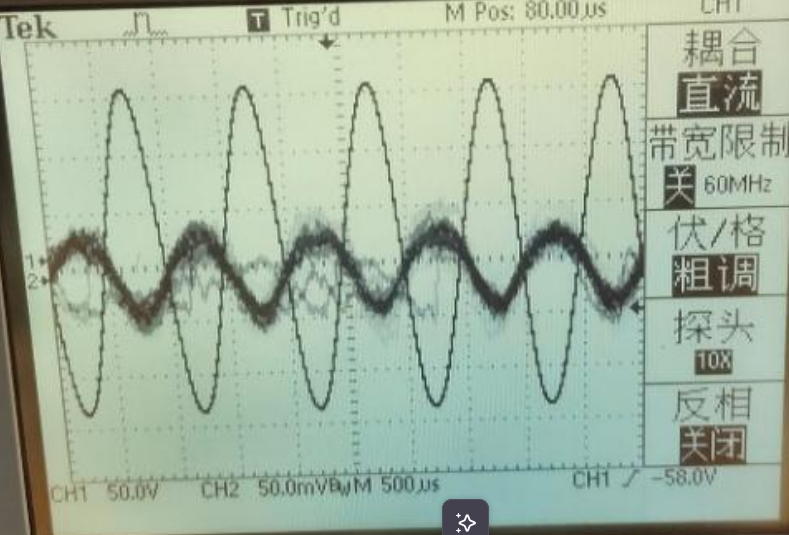
\includegraphics[width=0.7\linewidth]{217}
		\caption{$\theta=217^\circ$}
		\label{fig:217}
	\end{figure}
	\begin{figure}[H]
		\centering
		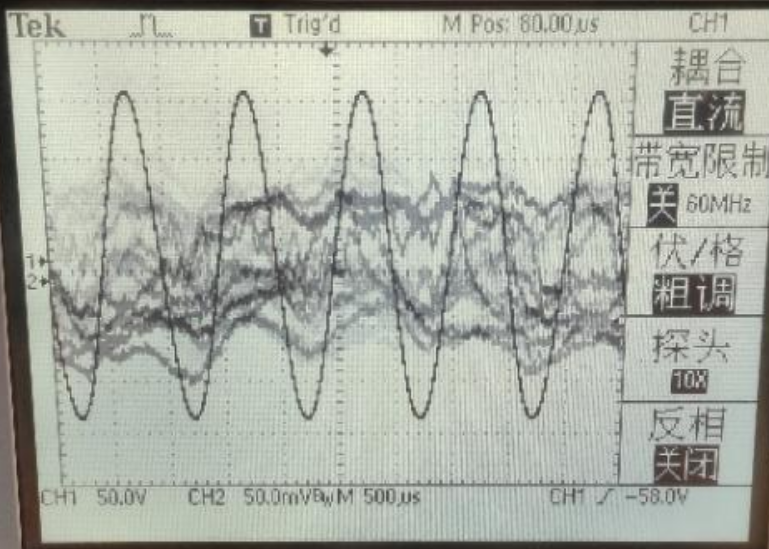
\includegraphics[width=0.7\linewidth]{275}
		\caption{$\theta=275^\circ$}
		\label{fig:275}
	\end{figure}
	\begin{figure}[H]
		\centering
		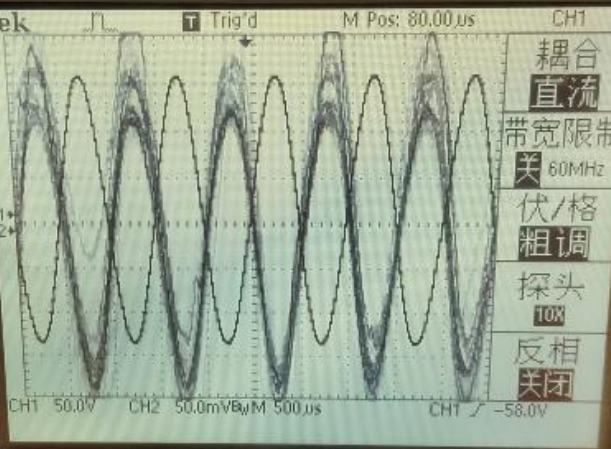
\includegraphics[width=0.7\linewidth]{303}
		\caption{$\theta=303^\circ$}
		\label{fig:303}
	\end{figure}
	
	\section{拟合分析}
	我们取 $\frac{V_m}{V_\pi} = 0.01$，在 $\frac{V_{DC}}{V_\pi}=\pm0.5,\ \pm0.25,\ 0$ 条件下画出曲线：
	\begin{equation}
		\begin{aligned}
			I &= \frac{1}{2}I_0\Bigl\{[1-\cos(\frac{\pi V_{DC}}{V_\pi})\cos(\frac{\pi V_m}{V_{\pi}}\sin\omega t)] \\
			&\quad + \sin(\frac{\pi V_{DC}}{V_\pi})\sin(\frac{\pi V_m}{V_\pi}\sin(\omega t))\Bigr\}
		\end{aligned}
	\end{equation}
	\begin{figure}[H]
		\centering
		
\includegraphics[width=0.7\linewidth]{0}
		\caption{$\frac{V_m}{V_\pi}=0.01,\ \frac{V_{DC}}{V_\pi}=0$，出现倍频调制现象}
		\label{fig:0}
	\end{figure}
	\begin{figure}[H]
		\centering
		
\includegraphics[width=0.7\linewidth]{0.5}
		\caption{$\frac{V_m}{V_\pi}=0.01,\ \frac{V_{DC}}{V_\pi}=0.5$}
		\label{fig:05}
	\end{figure}
	\begin{figure}[H]
		\centering
		
\includegraphics[width=0.7\linewidth]{-0.5}
		\caption{$\frac{V_m}{V_\pi}=0.01,\ \frac{V_{DC}}{V_\pi}=-0.5$}
		\label{fig:neg05}
	\end{figure}
	\begin{figure}[H]
		\centering
		
\includegraphics[width=0.7\linewidth]{0.25}
		\caption{$\frac{V_m}{V_\pi}=0.01,\ \frac{V_{DC}}{V_\pi}=0.25$}
		\label{fig:025}
	\end{figure}
	\begin{figure}[H]
		\centering
		
\includegraphics[width=0.7\linewidth]{-0.25}
		\caption{$\frac{V_m}{V_\pi}=0.01,\ \frac{V_{DC}}{V_\pi}=-0.25$}
		\label{fig:neg025}
	\end{figure}
	
	可以看出，光学偏压越大，输出光强调制范围越大（这一结论的前提是用 $\lambda/4$ 波片产生的光学偏压 $V_{DC} \in [-2\pi, 2\pi]$）。
	
	\begin{equation}
		I \approx \frac{I_0}{8}\left(\pi\frac{V_m}{V_\pi}\right)^2\left[1 - \cos(2\omega t)\right].
	\end{equation}
	上式表明输出光强包含直流分量和频率为 $2\omega$ 的交流分量，即输出信号频率为输入调制信号频率的两倍，此即\textbf{倍频调制现象}。
	
	\section{误差分析}
	我们利用误差的计算对第~\ref{sec:compare} 节中的计算结果进行误差分析。先计算 $r_{22}$ 的误差。
	
	电压的测量精确到个位：
	\begin{equation}
		u_{V_\pi}  = 0.577\ \text{V}
	\end{equation}
	\begin{equation}
		u_{r_{22}} = \left|\frac{\partial r_{22}}{\partial V_\pi}\right| u_{V_\pi} =  7.703604806\times10^{-4}\,u_{V_\pi}
	\end{equation}
	\begin{equation}
		r_{22} = (1 \pm 7.703604806\times10^{-4})\times6.219773031\times10^{-12}\ \text{m/V}
	\end{equation}
	
	再计算 $M$（消光比）的误差：
	\begin{equation}
		u_{I_{\max}^+} = u_{I_{\min}^+} = u_{I_{\max}^-} = u_{I_{\min}^-} = 5.773502692\times10^{-4}\ \text{mW}
	\end{equation}
	\begin{equation}
		M = \sqrt{\frac{I_{\max}^+ I_{\max}^-}{I_{\min}^+ I_{\min}^-}}
	\end{equation}
	\begin{equation}
		u_{M} = \sqrt{\sum_{A=\{\min,\max\},\ B=\pm}\left(\frac{\partial M}{\partial I_{A}^B}\,u_{I_{A}^B}\right)^2} = 0.482923
	\end{equation}
	则
	\begin{equation}
		M = 22.8 \pm 0.482923
	\end{equation}
	
	\begin{enumerate}
		\item 晶体光学均匀性、偏振片取向精度、入射光发散角与取向精度、外电场均匀性等因素都制约了我们对半波电压、消光比的测量精度。
		\item 电压与光功率的测量都是通过数字电表读数完成的，而数字信号本身的不连续性就会带来读数误差。
		\item 环境噪音会导致光路受到轻微扰动，进而影响光功率的实测值。
		\item 我们的理论推导本身就包含了近似，我们近似地认为折射率主轴旋转的角度与 $X_3$ 坐标无关，这个近似其实引入了系统误差。
	\end{enumerate}
\end{document}